\documentclass[11pt,letterpaper]{article}
\usepackage[utf8]{inputenc}
\usepackage[T1]{fontenc}
\usepackage[margin=1in]{geometry}
\usepackage{amsmath,amssymb}
\usepackage{graphicx}
\usepackage{hyperref}
\usepackage{xcolor}
\usepackage{enumitem}
\usepackage{caption}

\hypersetup{colorlinks=true,linkcolor=black,urlcolor=black,citecolor=black}
\graphicspath{{../figures/}}

\title{\textbf{The AI \texorpdfstring{$\times$}{x} Blockchain Intersection in Zoo}\\\large Why Both Layers Are Necessary, and What Each Provides}
\author{Antje Worring \\ \textit{Founder, Zoo Labs Foundation} \\ \texttt{antje@zoo.ngo}}
\date{October 31, 2021}

\begin{document}
\maketitle

\begin{abstract}
Zoo's animals are simultaneously AI agents and on-chain assets. This element paper explains the division of labour between the two layers as articulated in the founding whitepaper~\cite{zoo2021}. The blockchain provides identity, ownership, value-flow, and governance. The AI layer provides personality, conversation, and emotional resonance. Neither layer is sufficient alone.
\end{abstract}

\section{What blockchain provides}

\begin{itemize}
  \item \textbf{Identity.} Each animal is a distinct on-chain token with verifiable provenance.
  \item \textbf{Ownership.} Cryptographic ownership of a private key controls the animal.
  \item \textbf{Value-flow.} Collateralization, daily rewards, breeding fees, and burn refunds are all enforced by smart contracts.
  \item \textbf{Governance.} The Zoo DAO ratifies protocol changes including AI prompt updates and model curation.
  \item \textbf{Composability.} Standardized NFT interfaces allow any external service to integrate Zoo animals.
\end{itemize}

\section{What AI provides}

\begin{itemize}
  \item \textbf{Personality.} Each animal has a distinct character. The whitepaper~\cite{zoo2021} ships personality prompts for every life stage of every V1 species.
  \item \textbf{Conversation.} The animal responds to its owner in voice and register appropriate to its species and age.
  \item \textbf{Emotional resonance.} The AI is trained or steered to recognize emotional cues and respond empathetically. The animal becomes a digital companion, not a static collectible.
  \item \textbf{Adaptation.} Over time, the animal learns the owner's preferences and conversational style.
\end{itemize}

\section{Why neither layer suffices alone}

A pure-AI animal companion (no blockchain) lacks:

\begin{itemize}
  \item Cryptographic ownership: the user cannot truly own or transfer the animal.
  \item Verifiable scarcity: there is no way to ensure the rare animals stay rare.
  \item Conservation flow: there is no on-chain mechanism to route economic value to non-profit partners.
  \item Governance independence: prompt and model changes are at vendor whim.
\end{itemize}

A pure-NFT animal (no AI) lacks:

\begin{itemize}
  \item Personality and conversation.
  \item Emotional resonance.
  \item The metaverse-companion experience that justifies long-term holding beyond speculation.
\end{itemize}

\section{The integration surface}

The integration between the two layers happens at three points:

\begin{enumerate}
  \item \textbf{NFT metadata.} The on-chain metadata of the animal includes (or commits via hash to) the personality prompt that drives the AI.
  \item \textbf{Memory anchoring.} Long-term memories of conversations can be anchored on chain (or on a content-addressable storage layer with on-chain commitment) to survive vendor migrations of the AI implementation.
  \item \textbf{Governance hooks.} The DAO votes on prompt updates, model endorsements, and prompt-extension proposals. Votes are on chain, executed by smart contracts.
\end{enumerate}

\section{Failure modes the integration prevents}

\begin{enumerate}
  \item \textbf{The vendor sunset.} A pure-AI companion goes offline when the vendor pivots. Zoo's animal lives on as long as one provider runs the open prompt and one indexer surfaces the metadata.
  \item \textbf{The IP grab.} A vendor cannot claim ownership of a personality prompt that is recorded on chain by the holder.
  \item \textbf{The silent rug.} A vendor cannot quietly degrade the model. The DAO governs canonical model endorsement.
\end{enumerate}

\section{The 2021 commitment}

This integration was decided in 2021. It is the architectural reason Zoo can survive both crypto and AI hype cycles. When AI is up, Zoo's animals get smarter. When crypto is up, Zoo's economics flourish. When either is down, the other layer carries the project. This is risk diversification at the protocol level.

\begin{figure}[h]
\centering
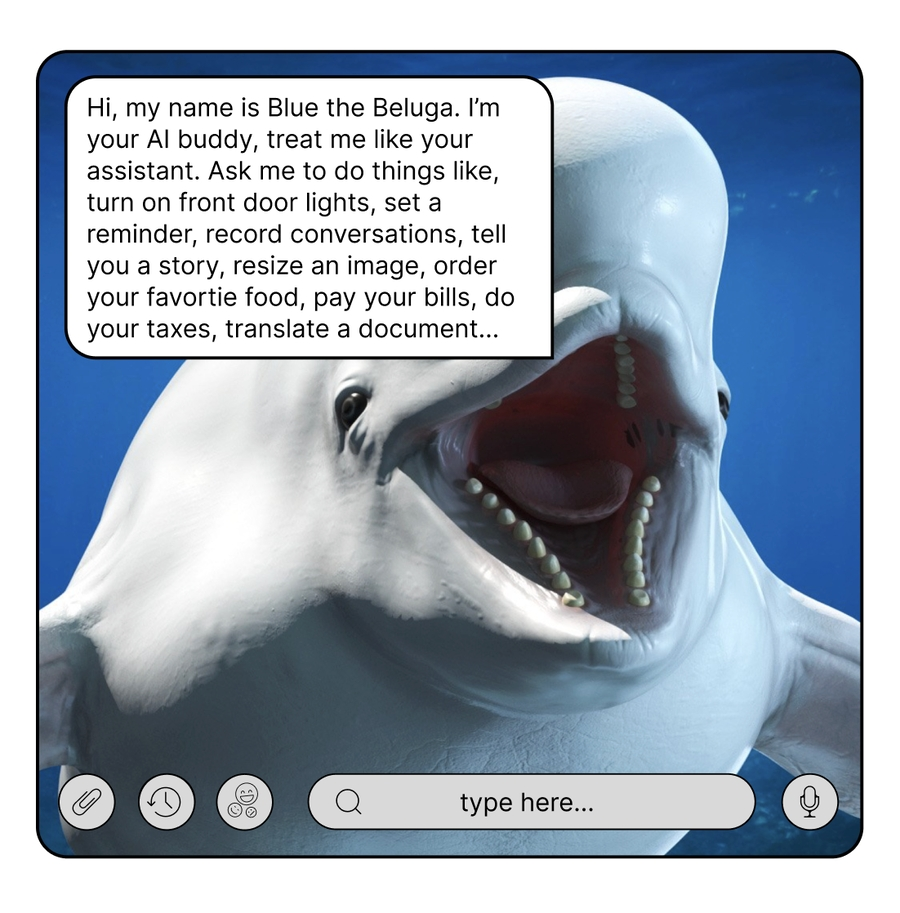
\includegraphics[width=0.55\textwidth]{ai-chat.png}
\caption{Reference UI of the Zoo AI assistant. The conversation surface is bound to a specific NFT identity --- the AI does not exist independently of the on-chain animal it represents.}
\end{figure}

\section{Bridging chains: what this enables}

The whitepaper~\cite{zoo2021} commits Zoo to be cross-chain by design. This affects the AI integration in two ways:

\begin{itemize}
  \item The animal's on-chain identity is anchored on a primary chain (initially Binance Smart Chain), but the metadata layer is portable across chains via the Zoo Bridge Protocol's threshold-signature scheme.
  \item Burning a Zoo animal on one chain to mint on another preserves the lineage memory described in the Open AI Protocol element paper. The personality survives the chain migration.
\end{itemize}

\section{Why blockchain governance matters for AI}

Recent industry experience demonstrates that closed-source AI companions are inherently fragile: the vendor can revise behavior without notice, sunset products on commercial whim, or restrict access regionally. Zoo's DAO governance of prompt updates and model curation is the antidote. A holder of a Zoo animal in 2021 expects that the same animal, addressable via the same on-chain identity, will be conversable on similar terms in 2031. The DAO governance hook makes that expectation enforceable.

\section{The animal as a financial primitive}

A Zoo animal is simultaneously:

\begin{enumerate}
  \item A liquidity-pool token with collateral backing and a daily yield curve.
  \item A breeding-rights certificate constrained by generational rules.
  \item An access pass to metaverse experiences and physical animal sanctuaries.
  \item An AI companion with a persistent personality.
\end{enumerate}

The AI \texttimes{} blockchain integration is what makes all four of these properties cohere into a single asset rather than four disjoint things.

\section{Concrete example: a year in the life}

Consider an Amur Leopard NFT minted on Day 0:

\begin{itemize}
  \item Day 0: Sublime Egg (1 ETH) is purchased. Egg metadata commits to species and rarity.
  \item Day 1: Egg hatches (free). Baby Whiskers personality activates. AI companion begins conversational relationship with holder.
  \item Day 60: Holder feeds 1 ETH to mint the teen form. Personality transitions to Flash. Memory carries forward.
  \item Day 180: Holder breeds Flash with another adult Amur Leopard, paying 3 ETH. New egg minted; lineage tracked.
  \item Day 365: Daily $\$ZOO$ rewards have accumulated. Holder may continue collateralizing for boost, sell, or burn.
\end{itemize}

At every step, the AI layer is contextually aware of the on-chain state of the animal. The animal's mood when its owner has just paid breeding fees is different from its mood after a year of accumulated rewards. \emph{The AI is aware of its on-chain state} --- this is what crosschain-AI fusion looks like in practice.

\begin{thebibliography}{1}
\bibitem{zoo2021} Antje Worring. \emph{Zoo: A Game-Fi Multiverse Ecosystem for the Preservation of Endangered Species}. Zoo Labs Foundation, October 31, 2021.
\end{thebibliography}

\end{document}
